\subsection{Análisis en el dominio del tiempo}

En la Figura \ref{fig:tiempo_rf} se observa la relación directa entre la señal modulante y la señal modulada en RF. La señal modulante presenta una forma rectangular binaria, mientras que la señal RF corresponde a una portadora senoidal cuya presencia depende del valor del bit.

Cuando la señal modulante es igual a 1, la portadora se transmite; cuando es 0, la portadora se suprime. Este comportamiento confirma que el sistema implementa correctamente una modulación OOK (On-Off Keying).

Adicionalmente, la representación en envolvente compleja muestra que la información se concentra en la componente en fase (I), mientras que la componente en cuadratura (Q) permanece en cero.

\begin{figure}[H]
\centering
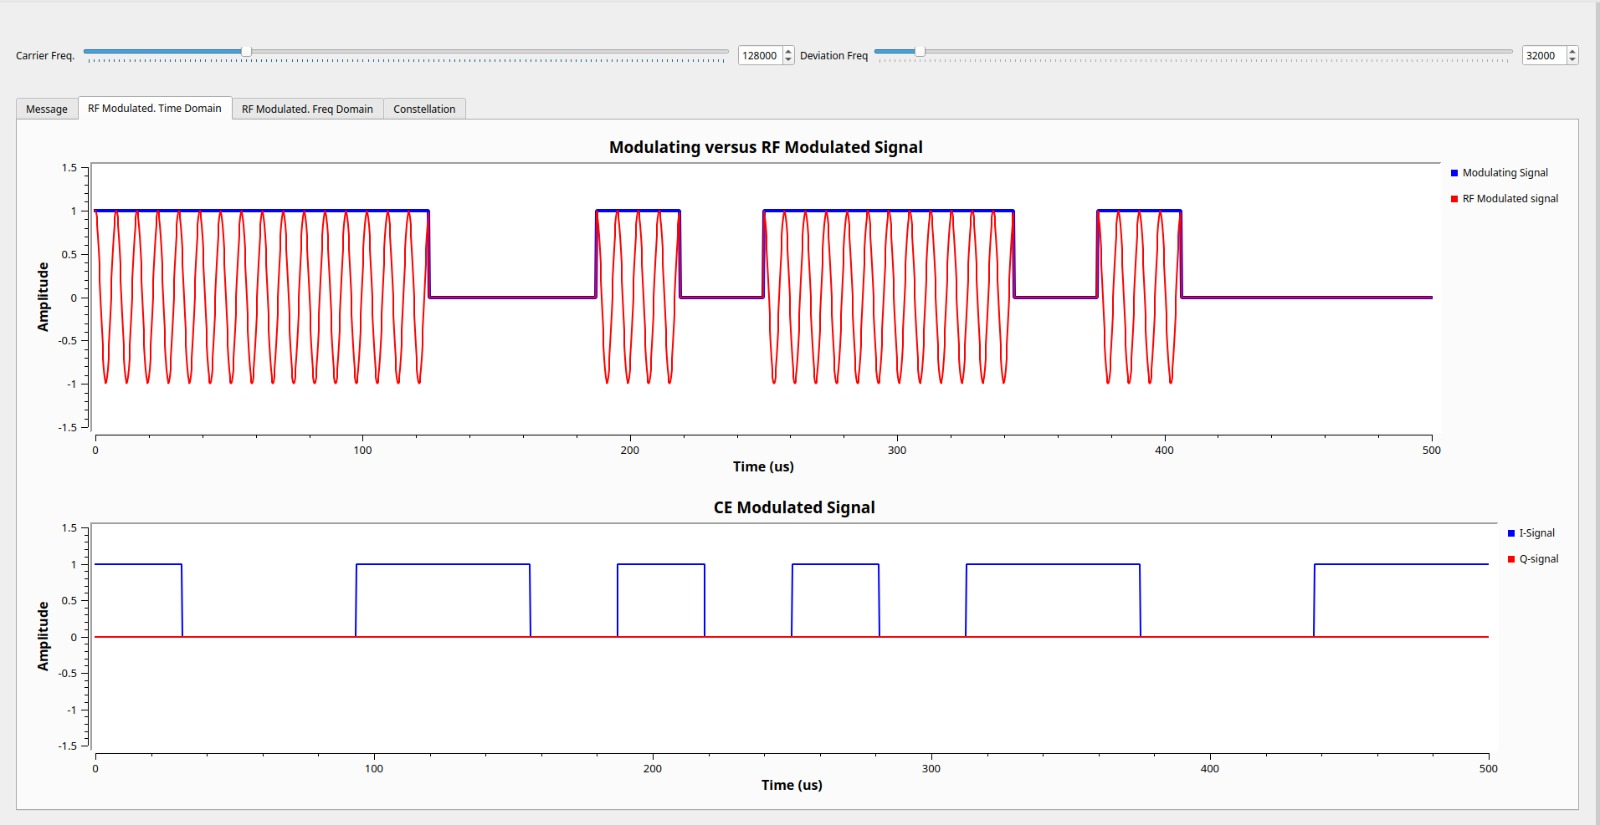
\includegraphics[width=0.48\textwidth]{imagenes/5.2.jpeg}
\caption{Señal modulada en RF comparada con la señal modulante y su representación en EC.}
\label{fig:tiempo_rf}
\end{figure}

\subsection{Análisis en el dominio de la frecuencia}

En la Figura \ref{fig:frecuencia_rf} se observa que la señal RF presenta su espectro centrado alrededor de la frecuencia portadora, con lóbulos laterales característicos. Esto corresponde al desplazamiento espectral de la señal base hacia la portadora.

Por otro lado, la señal en envolvente compleja presenta un espectro centrado en 0 Hz, conservando la misma forma espectral pero sin desplazamiento.

\begin{figure}[H]
\centering
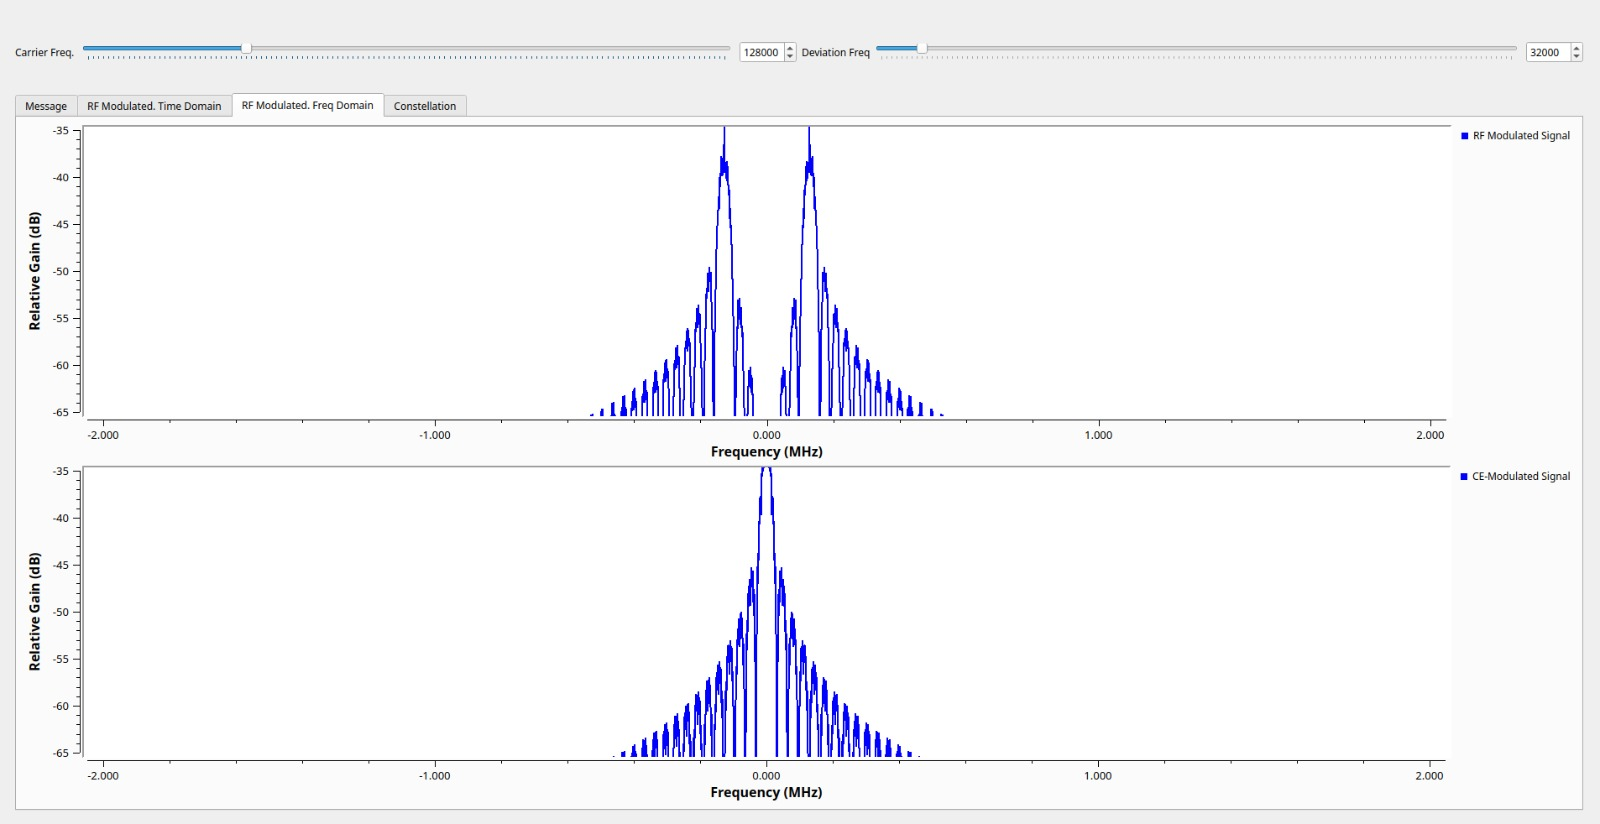
\includegraphics[width=0.48\textwidth]{imagenes/5.3.jpeg}
\caption{Comparación del espectro en RF y en envolvente compleja.}
\label{fig:frecuencia_rf}
\end{figure}

\subsection{Variación de la frecuencia portadora en el dominio del tiempo}

En la Figura \ref{fig:variacion_tiempo} se muestran las gráficas obtenidas al variar la frecuencia portadora. Se observa que, al aumentar la frecuencia, la señal RF presenta un mayor número de oscilaciones dentro de cada símbolo.

Sin embargo, la señal en envolvente compleja mantiene su forma, evidenciando que no depende directamente de la portadora.

\begin{figure}[H]
\centering
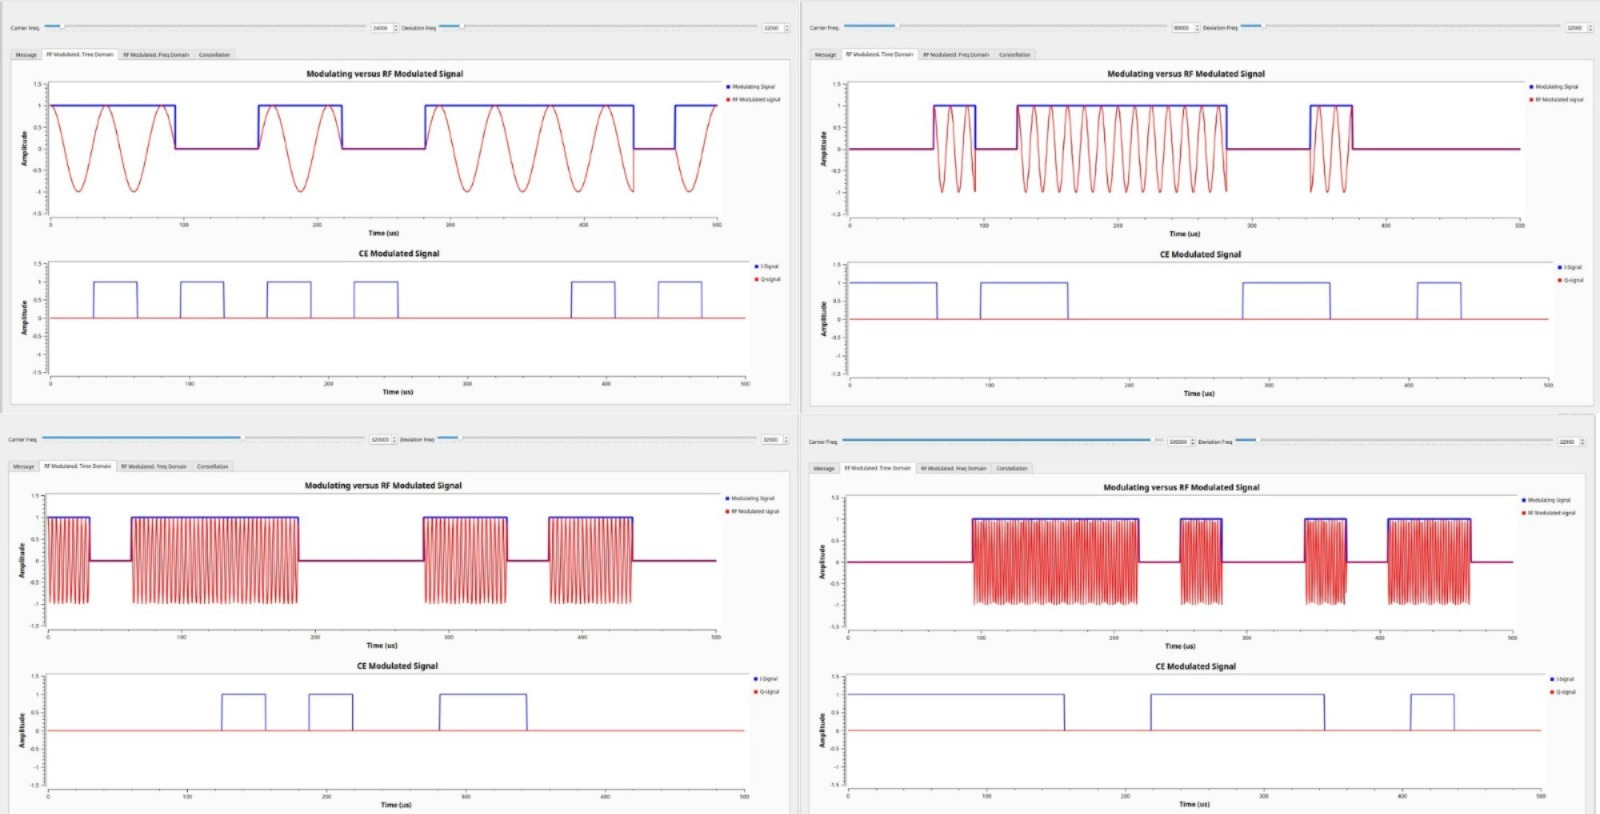
\includegraphics[width=0.48\textwidth]{imagenes/5.4.jpeg}
\caption{Variación de la señal en el dominio del tiempo al cambiar la frecuencia portadora.}
\label{fig:variacion_tiempo}
\end{figure}

\subsection{Variación de la frecuencia portadora en el dominio de la frecuencia}

En la Figura \ref{fig:variacion_freq} se observa que el espectro de la señal RF se desplaza proporcionalmente con la frecuencia portadora.

Por el contrario, el espectro de la señal en envolvente compleja permanece centrado en 0 Hz para todos los casos.

\begin{figure}[H]
\centering
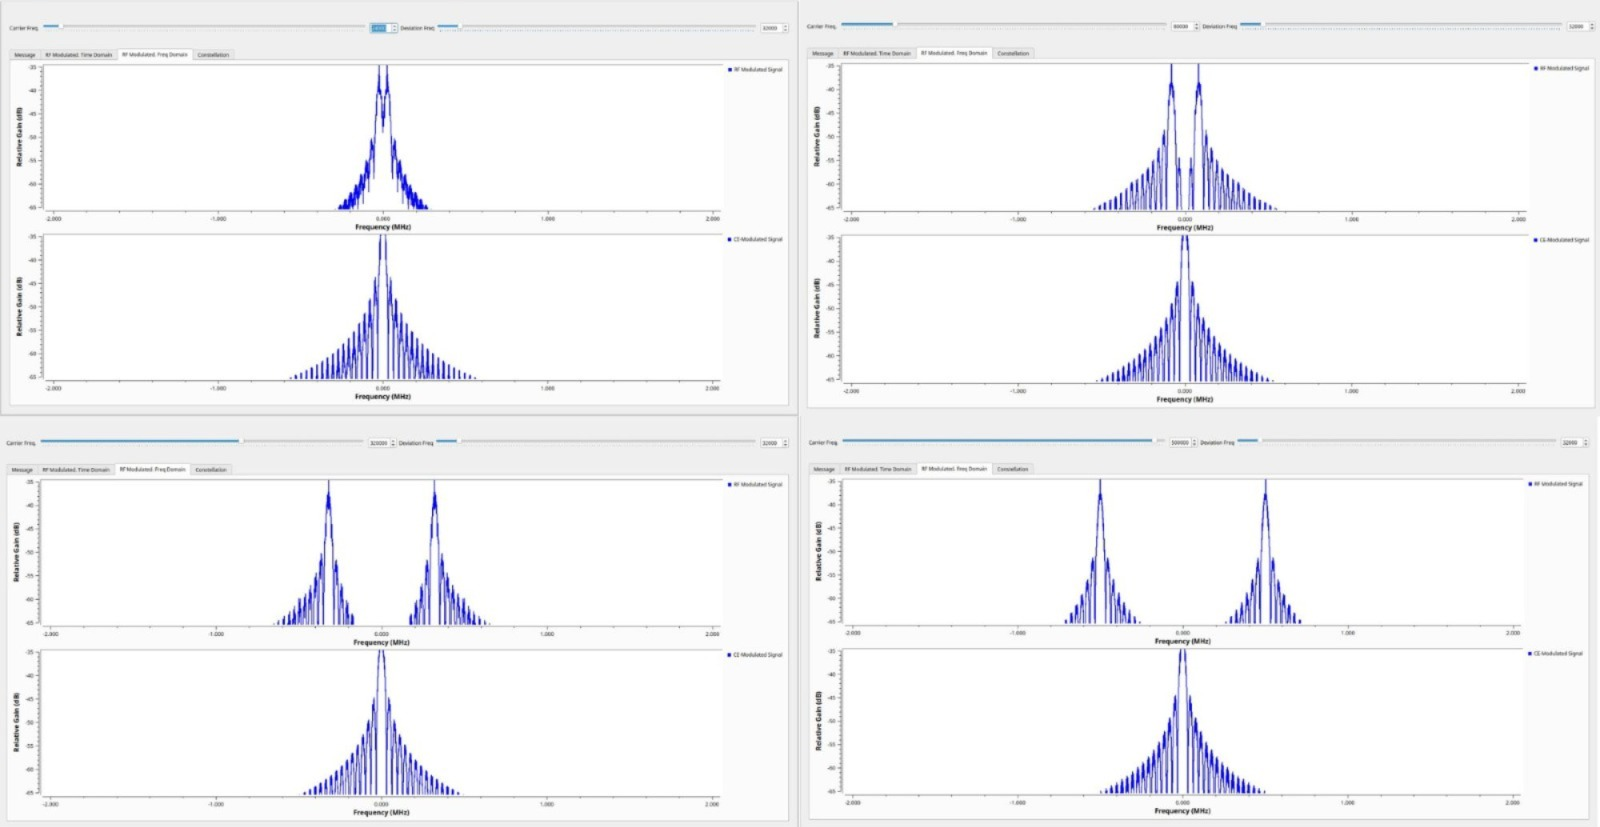
\includegraphics[width=0.48\textwidth]{imagenes/5.5.jpeg}
\caption{Desplazamiento espectral de la señal RF al variar la frecuencia portadora.}
\label{fig:variacion_freq}
\end{figure}

\subsection{Comparación entre OOK en RF y en EC}

A partir de los resultados obtenidos, se observa que ambas representaciones contienen la misma información, pero en dominios diferentes. En RF, la señal se representa como una portadora que se activa o desactiva, mientras que en EC la información se expresa en banda base mediante la envolvente.

Esto permite concluir que la representación en RF es adecuada para describir la transmisión física, mientras que la envolvente compleja resulta más eficiente para el análisis digital.



